\documentclass{article}
\usepackage[letterpaper, margin=1in]{geometry}
\usepackage[pdftex]{graphicx}
\usepackage[utf8]{inputenc}
\usepackage{tikz, wrapfig, amssymb, array, mathtools, enumitem, circuitikz, physics, parskip, hyperref}
\usepackage{tkz-euclide}
\usepackage{titlesec}
\usepackage{lipsum}
\usepackage[english]{babel}
\usepackage{amsmath, amsthm}
\usepackage{fancyhdr}
\usepackage{xcoffins}
\usepackage{dirtytalk}
\usepackage{tcolorbox}
\usepackage{../local}


\title{Physics 137A Homework}
\author{Yutong Du}


\begin{document}

\maketitle 

\section*{Collaborators}

I worked with \textbf{Andrew Binder} to complete this homework.

\section*{Problem 1}

Show that $[Ae^{ikx} + Be^{-ikx}]$ and $[C \cos kx + D \sin kx]$ are equivalent ways of writing the same function of $x$, and determine the constants $C$ and $D$ in terms of $A$ and $B$, and vice versa. 


\begin{solution}
    We can rewrite:

    \[ \begin{cases}
        Ae^{ikx} = A(\cos kx + i \sin kx)\\
        Be^{-ikx} = B(\cos kx - i \sin kx)
    \end{cases}\]

    So we can sum the two:

    \[ Ae^{ikx} + Be^{-ikx} = (A+B)\cos kx + (A - B)i \sin kx\]

    Here we get that $C = A+B$ and $D = (A-B)i$. If we were to define them the other way around, we would get $A = \frac{C - iD}{2}$ and $B = \frac{C + iD}{2}$.
\end{solution}

\pagebreak
\section*{Problem 2}

A Gaussian distribution, parametrised by $\mu$ and $\sigma$, is given by 

\[ \rho(x) = A \exp{-\frac{(x - \mu)^2}{2\sigma^2}}\]


\begin{enumerate}[label = (\alph*)]
\item Define 
\[ I = \infint e^{-x^2} \dx\]

Show that $I = \sqrt{\pi}$.

\begin{solution}
    The trick is to write this integral as the product of two identical integrals, using different variables for each:
    
    \begin{align*}
        I^2 &= \left(\infint e^{-x^2} \dx \right)\left(\infint e^{-y^2} dy\right)\\
        &= \infint e^{-(x^2 + y^2)} \dx \dd y
    \end{align*}

    Now we introduce a change of variables from cartesian to polar coordinates: 

    \begin{align*}
        I^2 &= \int_{-\pi}^\pi \int_0^\infty e^{-r^2} r \dd r \dd \theta\\
        &= \int_{-\pi}^\pi \dd \theta \int_0^\infty e^{u} \dd u\\
        &= 2\pi \cdot \frac{1}{2} e^u \bigg|_{-\infty}^0\\
        &= \pi
    \end{align*}

    And since $I^2 = \pi$, the it follows that $I = \sqrt{\pi}$.

\end{solution}


\item Hence find the normalization constant $A$.


\begin{solution}
    We use our result from part (a) by substituting $x \to \frac{x - \mu}{\sqrt{2}\sigma}$, meaning that our overall integral changes by a factor of $\frac{1}{\sqrt{2} \sigma}$.

    But then we need $\infint \rho(x) = 1$ so we have 

    \[ \frac{A\sqrt{\pi}}{\sqrt{2} \sigma} = 1 \implies A = \sqrt{\frac{2\sigma^2}{\pi}}\]


\end{solution}

\item Find $\mean{x}$, $\mean{x^2}$, $\sigma(x)$ of the given gaussian. %TODO


\begin{solution}
    We have $\mean{x} = \int x\rho(x) \dx$:

    \begin{align*}
        \mean{x} &= \infint x\exp{-\frac{(x-\mu)^2}{2\sigma^2}}\\
        &= \frac{\sqrt 2 \sigma}{\sqrt{\pi}} \infint x \exp{\frac{(x - \mu)^2}{2\sigma^2}} \dx\\
        &= \frac{\sqrt 2 \sigma}{\sqrt{\pi}} \infint (u + \mu) e^{-u^2}{2\sigma^2} \dd u\\
        &= \frac{\sqrt 2 \sigma}{\sqrt{\pi}} \left[\infint u \exp{-\frac{u^2}{2\sigma^2}} \dd u + \mu \infint \exp{\frac{-u^2}{2\sigma^2}} \dd u\right]
    \end{align*}

    The first integral is equal to zero, a result known from complex analysis. Our second integral is simply a variation of the one in part (a), so we can use the result from there to get:

    \[ \mean{x} = \frac{\sqrt 2 \sigma}{\sqrt{\pi}} \cdot \frac{\mu \sqrt \pi}{\sqrt{2} \sigma} = \mu\]

    A similar approach is applied to get $\mean{x^2}$: 


    \begin{align*}
        \mean{x^2} &= \infint x^2 A\exp{-\frac{(x-\mu)^2}{2\sigma^2}} \dx \\
        &= \frac{\sqrt \pi}{\sqrt{2} \sigma}\infint (u + \mu)^2 \exp{-\frac{u^2}{2\sigma^2}} \dd u\\
        &= \frac{\sqrt \pi}{\sqrt{2} \sigma} \left[\infint u^2 \exp{-\frac{u^2}{2\sigma^2}} \dd u + \mu \infint 2u\exp{-\frac{u^2}{2\sigma^2}} \dd u + \mu^2 \infint \exp{-\frac{u^2}{2\sigma^2}}\right]
    \end{align*}

    We use the hint to evaluate the first integral, the second integral is equal to zero just like in $\mean{x}$, and the third integral is our original gaussian:


    \begin{align*}
        \mean{x^2} &= -\frac{\partial}{\partial(\frac{1}{2\sigma^2})} \frac{\sqrt \pi}{\sqrt{2}\sigma} + \mu^2 \frac{\sqrt{\pi}}{\sqrt{2}\sigma}\\
        &= \frac{\sqrt \pi \sigma}{\sqrt{2}}\left(\mu^2 - 1\right)
    \end{align*}

    First, we can calculate $\sigma^2(x) = \mean{x^2} - \mean{x}^2$:

    \begin{align*}
        \sigma^2(x) &= \frac{\sqrt \pi \sigma}{\sqrt{2}}\left(\mu^2 - 1\right) - \mu^2\\
        \therefore \sigma(x) = \sqrt{\frac{\sqrt \pi \sigma}{\sqrt{2}}\left(\mu^2 - 1\right) - \mu^2}
    \end{align*}
\end{solution}
\item Sketch the gaussian. Indicate $\mu$ and $\sigma$ on your sketch or describe the effect of changing them.


\begin{solution}
    Changing $\mu$ shifts the gaussian so that its peak is at $x = \mu$, and shifting $\sigma$ affects the spread of the distribution. As $\sigma$ increases, the peak of the gaussian decreases and its width increases, and the opposite occurs when $\sigma$ decreases. Here's the image:
    \begin{center}
        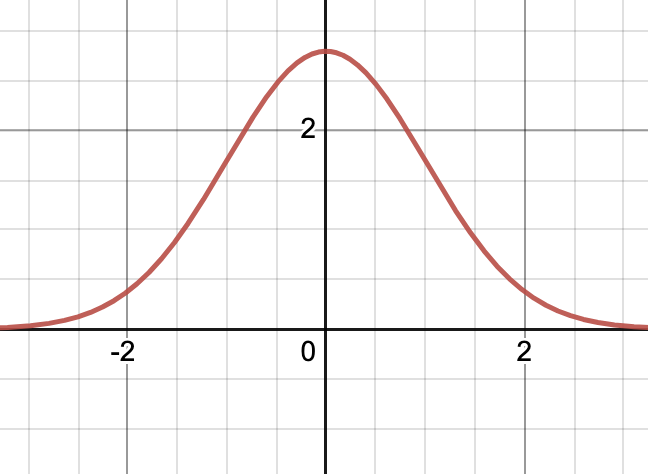
\includegraphics[scale=0.5]{gaussian.png}
    \end{center}
\end{solution}
\end{enumerate}

\pagebreak
\section*{Problem 3}

This problem is designed to guide you through a \say{proof} of Plancherel's theorem, by starting with the theory of ordinary Fourier series on a \textit{finite interval}, and allowing that interval expand to infinity. 

\begin{enumerate}[label=(\alph*)]
    \item Dirichlet's theorem says that \say{any} function $f(x)$ on the interval $[-a, +a]$ can be expanded as a fourier series:
    \[ f(x) = \sum_{n = 0}^\infty [a_n \sin (n\pi x/a) + b_n\cos(n\pi x/a)] \]

    Show that this is equivalently written as 

    \[ f(x) = \sum_{n = -\infty}^\infty c_ne^{in\pi x/a}\]

    What is $c_n$, in terms of $a_n$ and $b_n$?


    \begin{solution}
        We know from Euler's formula that $e^{ikx} = \cos(kx) + i \sin(kx)$, and by extension from problem 1, we can see that:

        \[ \frac{e^{ikx} + e^{-ikx}}{2} =\cos kx, \ \frac{e^{ikx} - e^{-ikx}}{2i} = \sin kx\]
        
        
        And thus we can rewrite our original expression:


        \begin{align*}
            f(x) &= \sum_{n = 0}^\infty \frac{a_n}{2i} \left(e^{in \pi x/a} - e^{-in\pi x/a}\right) + \frac{b_n}{2} \left(e^{in \pi x/a} + e^{-in \pi x/a}\right)\\
            &= \sum_{n = 0}^\infty \left(\frac{a_n}{2i} + \frac{b_n}{2}\right)e^{inx/a} + \sum_{n = 0}^\infty \left(\frac{b_n}{2} - \frac{a_n}{2i}\right)e^{-in\pi x/a}
        \end{align*}

        To reconcile the indices, we can let the latter take on values of $-n$, and as a result we can combine both terms: 


        \[ f(x) = \sum_{n = -\infty}^\infty \frac{b_n - ia_n}{2}e^{in \pi x/a}\]

        And thus giving us $c_n = \frac{b_n - ia_n}{2}$.
    \end{solution}


    \item Show (by appropriate modification of Fourier's trick) that 
    \[ c_n = \frac{1}{2a}\int_{-a}^{+a} f(x) e^{-in\pi x/a} \dx\]

    \begin{solution}
        We do discrete fourier transform on $a$:

        \begin{align*}
            \int_{-a}^a f(x) &= \int_{-a}^{a} \sum_{n = -\infty}^\infty c_n e^{in \pi x/a} \dx\\
            &= \sum_{n = -\infty}^\infty \int_{-a}^a c_ne^{in \pi x/a} \dx\\
        \end{align*}

        Note that thsi integral is equal to zero for any $n \neq 0$, so our sum effectively disappears, and we're left with the integral where $n = 0$:

        \[ \int_{-a}^a f(x) = c_0 \cdot 2a \implies c_0 = \frac{1}{2a}\int_{-a}^a f(x) \dx\]

        Thus, our general term becomes

        \[ c_n = \frac{1}{2a}\int_{-a}^a f(x) e^{-in \pi x/a} \dx\]



    \end{solution}

    


    \item Eliminate $n$ and $c_n$ in favor of the new variables $k = (n\pi / a)$ and $F(k) = \sqrt{2/\pi}a c_n$. Show that (a) and (b) now become
    \[ f(x) = \frac{1}{\sqrt{2\pi}}\sum_{n = -\infty}^\infty F(k)e^{ikx}\Delta k: F(k) = \frac{1}{\sqrt{2\pi}}\int_{-a}^a f(x) e^{-ikx} \dx\]

    where $\Delta k$ is the increment from one $n$ to the next. 

    \begin{solution}
        We know that $k = \frac{n\pi}{a}$ and $F(k) = \sqrt{2/\pi} ac_n$ so thus $c_n = \frac{F(k)}{\sqrt{2/\pi}a}$ and $n = \frac{ka}{\pi}$. First we can do $f(x)$: 


        \begin{align*}
            f(x) &= \sum_{n = -\infty}^\infty \frac{F(k)}{\sqrt{2/\pi} a} e^{-ikx}\\
            &= \sqrt{\frac{\pi}{2}} \sum_{n = -\infty}^\infty \frac{F(k)}{a} e^{ikx}
        \end{align*}

        Note that since in order to get the desired prefactor, we can multiply and divide by $\frac{\pi}{a}$:

        \begin{align*}
            f(x) &= \frac{1}{\sqrt{2\pi}} \sum_{n = -\infty}^\infty F(k) e^{-ikx} \frac{\pi}{a}
        \end{align*}

        Coincidentally, the step in $n$ is $\frac{\pi}{a}$, so therefore $\Delta k = \frac{\pi}{a}$. Thus:


        \[ f(x) = \frac{1}{\sqrt{2\pi}} \sum_{n = -\infty}^\infty F(k)e^{ikx} \Delta k\]

        As desired. Now we do $F(k)$:
        \begin{align*}
            \frac{F(k)}{\sqrt{2/\pi}a} &= \frac{1}{2a}\int_{-a}^a f(x) e^{-i\left(\frac{ka}{\pi}\right) \pi x/a} \dx\\
            F(k) &= \frac{\sqrt{2/\pi}}{2} \int_{-a}^a f(x) e^{-ikx} \dx\\
            &= \frac{1}{\sqrt{2\pi}} \int_{-a}^a f(x) e^{-ikx} \dx
        \end{align*}


        Which is what we wanted.
    \end{solution}
    
    \item Take the limit $a \to \infty$ to obtain Plancharel's theorem. 
    
    \begin{solution}
    Now we take $a \to \infty$, so that means that $k$ becomes a continuous variable, so our sum becomes an integral, thus:

    \begin{align*}
        f(x) &= \dfrac{1}{\sqrt{2\pi}}\infint F(k) e^{ikx} \dd k\\
        F(k) &= \dfrac{1}{\sqrt{2\pi}}\infint f(x) e^{ikx} \dx
    \end{align*}

    Which is precisely Plancahrel's theorem.

\end{solution}
\end{enumerate}

\pagebreak 


\section*{Problem 4}

A free particle has the initial wave function 

\[ \Psi(x, 0) = Ae^{-a|x|}\] 

where $A$ and $a$ are positive real constants.

\begin{enumerate}[label=(\alph*)]
\item Normalize $\Psi(x, 0)$. 


    \begin{solution}
        We know that the integral of the probability distribution must equal $1$:

        \begin{align*}
            1 &= \infint |\Psi(x, 0)|^2 \dx \\
            &= A^2 \infint \left|e^{-a|x|}\right|^2 \dx\\
            &= A^2\left[\int_{-\infty}^0 e^{2ax} \dx + \int_0^\infty e^{-2ax} \dx\right]\\
            &= A^2\left[\frac{1}{2a} + \frac{1}{2a} \right]\\
            &= \frac{A^2}{a}\\
            \therefore A &= \sqrt{a}
        \end{align*}

    \end{solution}
\item Find $\phi(k)$.

\begin{solution}
    Performing a continuous fourier transform:
    \[\phi(k) = \frac{\sqrt{a}}{\sqrt{2\pi}}\int_{-\infty}^{\infty}e^{-a|x|}e^{-ikx}dx = \sqrt{\frac{a}{2\pi}}\int_{-\infty}^{\infty}e^{-a|x|}(\cos(kx) - i\sin(kx))dx\]

    We can change the integral bounds because one of these functions will always be odd:

    \begin{align*}
        \phi(k) &= 2\sqrt{\frac{2}{2\pi}} \int_0^\infty e^{-ax} \cos kx \dx\\
        &= \sqrt{\frac{a}{2\pi}} \int_0^\infty \left[e^{(ik - a)x} + e^{-(ik + a)x} \right]\dx\\
        &= \sqrt{\frac{a}{2\pi}} \left[\frac{-ik - a + ik - a}{-k^2 - a^2}\right]\\
        &= \sqrt{\frac{a}{2\pi}}  \frac{2a}{k^2 + a^2}
    \end{align*} 
\end{solution}
\item Construct $\Psi(x, t)$, in the form of an integral.

\begin{solution}
    To get $\Psi(x, t)$, we combine what we've just got with the integral we found in lecture:

    \begin{align*}
        \Psi(x, t) &= \frac{1}{\sqrt{2 \pi}} \infint \exp{\frac{i(p_x x - E(p_x) t)}{\hbar}} \phi(p_x) \dd p_x\\
        &= \frac{\sqrt 2}{\sqrt{2\pi}} \sqrt{\frac{a^3}{2\pi}} \infint \frac{1}{k^2 + a^2} \exp{i\left(kx - \frac{\hbar k^2}{2m}t\right)}
    \end{align*}

    
\end{solution}
\item Discuss the limiting cases ($a$ very large, $a$ very small)

\begin{solution}
    For very large $a$, the amplitude of our wave function will grow very large, so we'll have large spikes in $\Psi(x, t)$, meaning that we will have meaning that we will have high certainty in our position but very little certainty of our momentum. The opposite would be true for small $a$.
\end{solution}
\end{enumerate}
\end{document}